\documentclass[preprint,12pt]{elsarticle}
\usepackage[utf8]{inputenc}
\usepackage[T1]{fontenc}
\usepackage{lmodern}
\usepackage{amsmath,amssymb}
\usepackage{graphicx}
\usepackage{booktabs}
\usepackage{multirow}
\usepackage{enumitem}
\usepackage{xcolor}
\usepackage{tikz}
\usetikzlibrary{calc,positioning,arrows.meta}
\usepackage[most]{tcolorbox}
\usepackage{listings}
\usepackage{url}
\usepackage[hidelinks]{hyperref}
\usepackage{lineno}
\graphicspath{{figures/}}
\newcommand{\npapers}{3,274}
\newcommand{\npapersIncluded}{3,117}
\newcommand{\npapersThreeDCP}{1,176}
\newcommand{\nmixes}{29,626}
\newcommand{\nmeasurements}{236,199}
\newcommand{\nmeasurementsValued}{81,030}
\newcommand{\ncurves}{25,721}
\newcommand{\ncurvePoints}{155,211}
\newcommand{\nprintRuns}{7,420}
\newcommand{\nprintPapers}{928}
\newcommand{\nprintPrintable}{5,586}
\newcommand{\nprintNon}{902}
\newcommand{\nprintBorder}{932}
\newcommand{\nprintCollapses}{941}
\newcommand{\nprintSTF}{841}
\newcommand{\nprotocolRows}{1,507}
\newcommand{\nnMixesNorm}{28,001}
\newcommand{\nnFeatures}{138}
\newcommand{\nnModels}{36}
\newcommand{\nnTargets}{19}
\newcommand{\nrFailN}{146}
\newcommand{\nrFailPapers}{37}
\newcommand{\nrFailMedian}{1.39}
\newcommand{\nrFailPtf}{0.64}
\newcommand{\nrFailPsf}{2.87}
\newcommand{\nnTools}{16}
\newcommand{\nbenchCxN}{33}
\newcommand{\nbenchCxPassn}{33}
\newcommand{\nbenchCxPassrate}{1.000}
\newcommand{\nbenchCxToolok}{33}
\newcommand{\nbenchCxParamok}{33}
\newcommand{\nbenchCxNchecks}{105}
\newcommand{\nbenchCxFidelity}{0.996}
\newcommand{\nbenchCxNnumbers}{497}
\newcommand{\nbenchCxNuntraced}{6}
\newcommand{\nbenchCxCallsmedian}{3}
\newcommand{\nbenchCxToolerrors}{6}
\newcommand{\nbenchCxWallmedian}{39}
\newcommand{\nbenchCxWallpninety}{89}
\newcommand{\nbenchCxWallmax}{172}
\newcommand{\nbenchCxCost}{0}
\newcommand{\nbenchCxModel}{gpt-6-astra}
\newcommand{\nbenchCxIntokens}{6,203,134}
\newcommand{\nbenchCxOuttokens}{32,650}
\newcommand{\nbenchCxCachetokens}{5,389,952}
\newcommand{\nbenchCxControl}{0.378}
\newcommand{\nbenchCxTruthn}{6}
\newcommand{\nbenchCxTruthok}{6}
\newcommand{\nbenchCxFatal}{0}
\newcommand{\nbenchCsN}{33}
\newcommand{\nbenchCsPassn}{33}
\newcommand{\nbenchCsPassrate}{1.000}
\newcommand{\nbenchCsToolok}{33}
\newcommand{\nbenchCsParamok}{33}
\newcommand{\nbenchCsNchecks}{105}
\newcommand{\nbenchCsFidelity}{0.998}
\newcommand{\nbenchCsNnumbers}{596}
\newcommand{\nbenchCsNuntraced}{4}
\newcommand{\nbenchCsCallsmedian}{4}
\newcommand{\nbenchCsToolerrors}{6}
\newcommand{\nbenchCsWallmedian}{48}
\newcommand{\nbenchCsWallpninety}{111}
\newcommand{\nbenchCsWallmax}{142}
\newcommand{\nbenchCsCost}{0}
\newcommand{\nbenchCsModel}{gpt-6-sol}
\newcommand{\nbenchCsIntokens}{7,150,793}
\newcommand{\nbenchCsOuttokens}{55,050}
\newcommand{\nbenchCsCachetokens}{6,284,288}
\newcommand{\nbenchCsControl}{0.445}
\newcommand{\nbenchCsTruthn}{6}
\newcommand{\nbenchCsTruthok}{6}
\newcommand{\nbenchCsFatal}{0}
\providecommand{\nbenchCxModel}{(pending)}

% ---------------------------------------------------------------- transcript boxes
\definecolor{userbg}{HTML}{FFF4D6}
\definecolor{agentbg}{HTML}{F3F4F6}
\definecolor{toolbg}{HTML}{E8F1FB}
\newtcolorbox{userbox}{enhanced, colback=userbg, colframe=userbg!60!black, boxrule=0.4pt, arc=2pt, left=5pt, right=5pt, top=3pt, bottom=3pt,
  fontupper=\small, title={\footnotesize\bfseries User}, attach title to upper={\ \ }, coltitle=black}
\newtcolorbox{agentbox}{enhanced, colback=agentbg, colframe=agentbg!55!black, boxrule=0.4pt, arc=2pt, left=5pt, right=5pt, top=3pt, bottom=3pt,
  fontupper=\small, title={\footnotesize\bfseries Agent}, attach title to upper={\ \ }, coltitle=black, breakable}
\newtcolorbox{mcpbox}[1]{enhanced, colback=white, colframe=black!50, boxrule=0.4pt, arc=1pt, left=3pt, right=3pt, top=2pt, bottom=2pt,
  title={\footnotesize\bfseries #1}, coltitle=white, colbacktitle=black!60}
\newtcolorbox{toolbox}[1]{enhanced, colback=toolbg, colframe=toolbg!70!black, boxrule=0.3pt, arc=1pt, left=3pt, right=3pt, top=1pt, bottom=0pt, boxsep=1pt,
  title={\footnotesize tool \texttt{#1}}, coltitle=black, colbacktitle=toolbg, toptitle=1pt, bottomtitle=0pt, before skip=3pt, after skip=3pt}
\newcommand{\toolmore}[1]{\par\noindent{\footnotesize\itshape\ \ \ldots\ #1 further tool calls omitted}\par\smallskip}
\lstdefinestyle{argstyle}{basicstyle=\ttfamily\scriptsize, breaklines=true, breakatwhitespace=false, columns=fullflexible, keepspaces=true, showstringspaces=false, frame=none, aboveskip=0pt, belowskip=0pt, extendedchars=true}
\usepackage{capt-of}
\usepackage{adjustbox}
\newcommand{\casefigure}[3]{\par\medskip\noindent\begin{tcolorbox}[enhanced, breakable, colback=white, colframe=black!35, boxrule=0.4pt, arc=2pt, left=4pt, right=4pt, top=4pt, bottom=4pt]\input{#1}\end{tcolorbox}\vspace{-6pt}\captionof{figure}{#2}\label{#3}\par\medskip}
\newcommand{\sessionsep}[1]{\par\medskip\noindent{\footnotesize\bfseries --- #1 ---}\par\smallskip}
\lstdefinestyle{jsonstyle}{basicstyle=\ttfamily\scriptsize, breaklines=true, breakatwhitespace=false, columns=fullflexible, keepspaces=true, showstringspaces=false, frame=none, extendedchars=true, literate={≥}{{$\geq$}}1 {≤}{{$\leq$}}1 {→}{{$\rightarrow$}}1 {τ}{{$\tau$}}1 {ρ}{{$\rho$}}1 {–}{{--}}1 {·}{{$\cdot$}}1 {²}{{$^2$}}1 {³}{{$^3$}}1 {µ}{{$\mu$}}1 {°}{{$^\circ$}}1 {±}{{$\pm$}}1 {×}{{$\times$}}1 {✅}{{[ok]}}4 {⚠}{{[!]}}3 {❌}{{[x]}}3 {’}{{'}}1 {“}{{``}}1 {”}{{''}}1}

\journal{Automation in Construction}

\begin{document}
\begin{frontmatter}

\title{3DCP-Agent: an LLM agent for planning and evaluating 3D concrete printing through natural-language access to literature-trained prediction, inverse mix design and buildability assessment}

\author[skku]{Solmoi Park\corref{cor1}}
\ead{solmoipark@skku.edu}
\cortext[cor1]{Corresponding author.}
\address[skku]{School of Civil, Architectural Engineering and Landscape Architecture, Sungkyunkwan University, Suwon, Republic of Korea}

\begin{abstract}
Planning a 3D concrete printing (3DCP) job means answering, in sequence, questions that today live in different tools and different experts: what fresh and hardened properties a candidate mix will have, which published mixes have reached a target, whether a given material will stand under a given nozzle, geometry and schedule, and which mix would. This paper presents 3DCP-Agent, in which a large language model (LLM) is the interface and the planner, while every number comes from validated computational tools: \nnModels{} property models trained on a literature database of \npapers{} papers (\nmixes{} mixes, \nmeasurements{} measurements, \ncurves{} digitised curves) with paper-grouped cross-validation and conformal 80\,\% intervals; an inverse mix-design engine; a physics-based buildability calculator (Roussel plastic collapse with linear structuration, Suiker free-wall buckling, open time) calibrated on \nprintRuns{} published print runs; literature retrieval; and read-only SQL over both databases. The \nnTools{} tools are defined once in a registry and projected to the Anthropic, OpenAI and Model Context Protocol (MCP) schemas, so the same agent runs on API keys or on a user's Claude or ChatGPT subscription, in a chat web application, a terminal, or any MCP client. Guardrails in the system prompt forbid numbers that did not come from a tool, require intervals and units, and require stated defaults. Case studies show end-to-end print planning in conversation: per-cubic-metre batch sheets are converted to mix specifications, buildability verdicts come with layer cycle-time windows and alternatives, and a print job is turned into ranked mix candidates with published analogues. A benchmark of 33 natural-language tasks measures tool selection, parameter extraction against expected values, ground-truth answers for database questions, refusal of unsupported requests, resistance to write attempts, and numeric fidelity (the fraction of numbers in an answer traceable to a tool result). The agent and the evaluation harness are released with the package.
\end{abstract}

\begin{keyword}
3D concrete printing \sep large language model \sep agent \sep tool use \sep model context protocol \sep mix design \sep buildability \sep literature database
\end{keyword}
\end{frontmatter}

\linenumbers

% =====================================================================================================================
\section{Introduction}

Extrusion-based 3D concrete printing (3DCP) couples material design to process design more tightly than any conventional casting method. A printable mortar must be pumpable and extrudable at the nozzle, must carry the layers placed on top of it before it sets, and must still deliver strength, shrinkage and durability in the hardened state \cite{buswell2018roadmap,roussel2018rheological}. The decisions a practitioner has to make are therefore distributed over several questions: what fresh and hardened properties a candidate mix is likely to have; which published mixes have already reached a given combination of targets; whether a given material will stand under a given nozzle, geometry and layer cycle time; and, in the inverse direction, which mix and which schedule a given object requires. Each of these questions has, by now, a quantitative answer in the literature: data-driven property models \cite{malik2024mixdesign3dcp,zafar2025ensemblerheology,ali2023mltensile3dcp,monkman2026datadrivenreview}, analytical buildability criteria \cite{roussel2018rheological,perrot2016structural,suiker2018mechanical,wolfs2018early,kruger2019lowerbound} and large collections of published mix designs. In practice, however, the answers sit in separate scripts, spreadsheets and papers, each with its own input format and its own vocabulary, so the questions are rarely asked together and almost never by the people who print.

Large language models (LLMs) have changed what an interface to such tools can be. An LLM can read a mix description written the way a laboratory writes it (``500 kg cement, 150 kg fly ash, 1300 kg sand, 227 kg water per cubic metre''), convert it into the structured input a model expects, decide which computation answers the question, call it, and explain the result. Tool use (function calling) and the Model Context Protocol (MCP) \cite{schick2023toolformer,yao2023react,anthropic2024mcp,hou2025mcp} make this orchestration reliable enough for engineering use, provided that the numbers themselves are produced by validated tools and not by the language model \cite{bran2024chemcrow}. Construction research has started to adopt this pattern for building information modelling, robotics, pavement management and structural health monitoring \cite{du2026text2bim,dong2025aibim,chen2025multiagentrc,zeng2026pavementagents,liu2026llm4shm,avila2025hai}, but not yet for the material-and-process planning problem of 3DCP, where the relevant tools are prediction models and physics calculators rather than databases and CAD.

This paper presents such an agent, which we call 3DCP-Agent. It is built on an open package that we developed for cement paste and mortar property prediction and inverse mix design from a validated literature database, and on a buildability layer calibrated on published print runs. The contribution of the present paper is the agent layer and its evaluation:

\begin{enumerate}[nosep]
\item \textbf{A tool registry that makes the computational layer callable by any LLM.} \nnTools{} tools (prediction, rheology curves, literature retrieval, inverse design, buildability and schedule, job-to-mix design, schema inspection and read-only SQL, report and memory) are defined once with a JSON schema and projected to the Anthropic, OpenAI and MCP schemas. The same agent therefore runs on an API key, on a Claude subscription through the Claude Agent SDK, or on a ChatGPT subscription through the Codex CLI, and can be attached as an MCP server to third-party clients.
\item \textbf{A print-planning conversation as a closed loop.} A print job described in words (object, height, nozzle, speed, open time) is checked against a measured or predicted material with Roussel/Perrot/Suiker criteria and the empirical collapse statistics of \nprintRuns{} published runs; when it fails, the agent reports the layer cycle-time window and the required static yield stress or structuration rate; and the job can be turned into a design specification whose candidates are re-assessed against the job.
\item \textbf{Guardrails and a measurable notion of faithfulness.} The system prompt forbids any quantitative statement that did not come from a tool result in the same conversation, requires predictions as $q_{50}\,[q_{10}, q_{90}]$ with units, and requires every default the agent filled in to be stated. We operationalise this as \emph{numeric fidelity}, the fraction of numbers in an answer that can be traced to the prompt, a tool input or a tool result, and measure it on every task.
\item \textbf{A reproducible benchmark.} 33 tasks in ten groups, each with machine-checkable expectations (tools called, parameters extracted, ground-truth answers for database questions, refusal of an unsupported property, rejection of a write attempt, persistence of a remembered preference), are run from a fresh session on each backend and scored without human judgement; the harness and the tasks are part of the released package.
\end{enumerate}

The remainder of the paper reviews related work (Section~\ref{sec:related}), describes the data and computational layer, the agent and the implementation (Section~\ref{sec:method}), presents case studies and the benchmark (Section~\ref{sec:results}), discusses limitations (Section~\ref{sec:discussion}) and concludes (Section~\ref{sec:conclusion}).

% =====================================================================================================================
\section{Related work}\label{sec:related}

\subsection{Tool-using LLM agents and the Model Context Protocol}

Toolformer showed that a language model can learn when to call external tools and how to use their results \cite{schick2023toolformer}; ReAct interleaves reasoning traces with actions and observations so that a model plans, acts and revises in one loop \cite{yao2023react}. Function calling, the production form of these ideas, lets a model emit a structured call against a JSON schema and receive the result as a message. In chemistry, ChemCrow demonstrated that an LLM equipped with expert tools solves synthesis and design tasks that the bare model cannot, and that the value lies in the tools, not in the model's recollection of facts \cite{bran2024chemcrow}. Retrieval-augmented generation addresses the complementary problem of grounding text answers in documents \cite{gao2023rag}. The Model Context Protocol, released in November 2024, standardises how a host application discovers and invokes tools, resources and prompts offered by a server, so that one server can be used by many clients and one client can combine many servers \cite{anthropic2024mcp,hou2025mcp}. The present work uses all three mechanisms: function calling against a registry, MCP for clients we do not control, and a lightweight retrieval of published analogue mixes.

\subsection{LLMs and agents in construction and civil engineering}

Table~\ref{tab:related} summarises recent construction-domain systems. Text2BIM generates and edits building models from natural language through multi-agent code generation \cite{du2026text2bim}; Dong et al.\ combine an LLM with BIM tooling for AI-assisted modelling \cite{dong2025aibim}; Gao et al.\ query and manipulate IFC models through an agent \cite{gao2026ifcagent}; Chen and Bao orchestrate robotic construction with several agents \cite{chen2025multiagentrc}; Ren et al.\ apply agentic control in engineering informatics \cite{ren2026agenticontrol}; Zeng et al.\ use agents for pavement management \cite{zeng2026pavementagents}; Liang et al.\ address structural engineering tasks \cite{liang2026llmstructural}. Closest to our setting are two MCP-based systems: Avila et al.\ connect GPT-4 to OpenSeesPy for structural analysis \cite{avila2025hai}, and Liu et al.\ build a multi-agent system for dam structural health monitoring in which the LLM orchestrates deep-learning behaviour models, an anomaly detector, a data-management agent and a RAG knowledge base through MCP \cite{liu2026llm4shm}. In the materials domain, LLMs have mostly been used for information extraction from the literature \cite{dagdelen2024structured,polak2024extracting,jablonka2023fourteen,li2026llmconcreteextraction} or evaluated as question-answering assistants \cite{li2024chatgptunderground}; direct LLM design of concrete has been proposed in a preprint \cite{volker2024llmconcrete} and LLMs have been combined with vision for process monitoring \cite{li2025concretevibrationllm} and with ML strength models \cite{zaman2026concretellm}. None of these systems gives an LLM tool access to property prediction, inverse design and buildability physics for 3DCP, and none reports a task-level benchmark of the agent layer itself; the dam-monitoring and structural-analysis papers evaluate their systems through case studies.

\begin{table}[t]
\centering\small
\caption{Recent LLM systems in construction and materials, and the present work. KB: knowledge base; MCP: model context protocol.}
\label{tab:related}
\resizebox{\textwidth}{!}{\begin{tabular}{p{3.0cm}p{3.2cm}p{3.4cm}cccp{2.4cm}}
\toprule
Reference & Domain & LLM role & Tools & MCP & KB & Evaluation \\
\midrule
Du et al.\ \cite{du2026text2bim} & BIM authoring & multi-agent code generation & yes & no & no & case + metrics \\
Dong et al.\ \cite{dong2025aibim} & BIM modelling & assistant & yes & no & no & case \\
Gao et al.\ \cite{gao2026ifcagent} & IFC querying & agent & yes & no & no & case + metrics \\
Chen, Bao \cite{chen2025multiagentrc} & robotic construction & multi-agent orchestration & yes & no & no & case \\
Zeng et al.\ \cite{zeng2026pavementagents} & pavement management & multi-agent & yes & no & yes & case \\
Avila et al.\ \cite{avila2025hai} & structural analysis & GPT-4 + OpenSeesPy & yes & yes & no & case \\
Liu et al.\ \cite{liu2026llm4shm} & dam SHM & orchestrator of 4 agents & yes & yes & RAG & case, timing \\
Li et al.\ \cite{li2024chatgptunderground} & underground concrete & Q\&A & no & no & no & expert rating \\
V\"olker et al.\ \cite{volker2024llmconcrete} & concrete mix design & direct generation & no & no & no & lab tests (preprint) \\
\textbf{This work} & 3DCP planning & planner + interface over validated tools & \nnTools{} & yes & 2 DBs & cases + 33-task benchmark \\
\bottomrule
\end{tabular}}
\end{table}

\subsection{Data-driven mix design and buildability in 3DCP}

Machine learning for 3DCP has mostly targeted single properties: slump flow and printability \cite{malik2024mixdesign3dcp}, rheology from small datasets with ensembles \cite{zafar2025ensemblerheology}, interlayer tensile strength \cite{ali2023mltensile3dcp}, bond and reinforcement design \cite{ma2024trustworthyml3dcp}, and generative design of printable mixes \cite{wang2024deepgenerative3dcp}; Monkman et al.\ review data-driven mix design and note the shortage of large, consistently extracted datasets \cite{monkman2026datadrivenreview}. Buildability has an analytical core: the bottom layer of a stack yields when its vertical stress exceeds $\sqrt{3}$ times the static yield stress, which itself grows during the print \cite{roussel2018rheological,perrot2016structural,reiter2018role}; slender walls fail earlier by elastic buckling \cite{suiker2018mechanical,wolfs2018early}; Kruger et al.\ formulated a lower-bound model and characterised thixotropy for these criteria \cite{kruger2019lowerbound,kruger2019thixotropy}. Our computational layer implements these criteria and calibrates them on published collapse tests; what is new here is that they are reachable through conversation together with the prediction models that supply their inputs.

% =====================================================================================================================
\section{Methodology}\label{sec:method}

\subsection{Overview}

Figure~\ref{fig:arch} shows the five layers of the system. Users reach the agent through a chat web application, a terminal, or an external MCP client. The agent core builds a system prompt with live context, runs the tool loop, and keeps session memory. All tools are defined once in a registry and projected to the schema each LLM backend expects. The computational layer is the existing prediction and design package: property models, inverse design, buildability physics, literature retrieval and guarded SQL. The data layer holds the literature database and the print-process database. The LLM never computes a property; it decides which tool to call with which arguments, and it explains the results.

\begin{figure}[p]
\centering
\resizebox{\textwidth}{!}{% System architecture (TikZ). Included from main.tex inside a figure environment (resized to \textwidth).
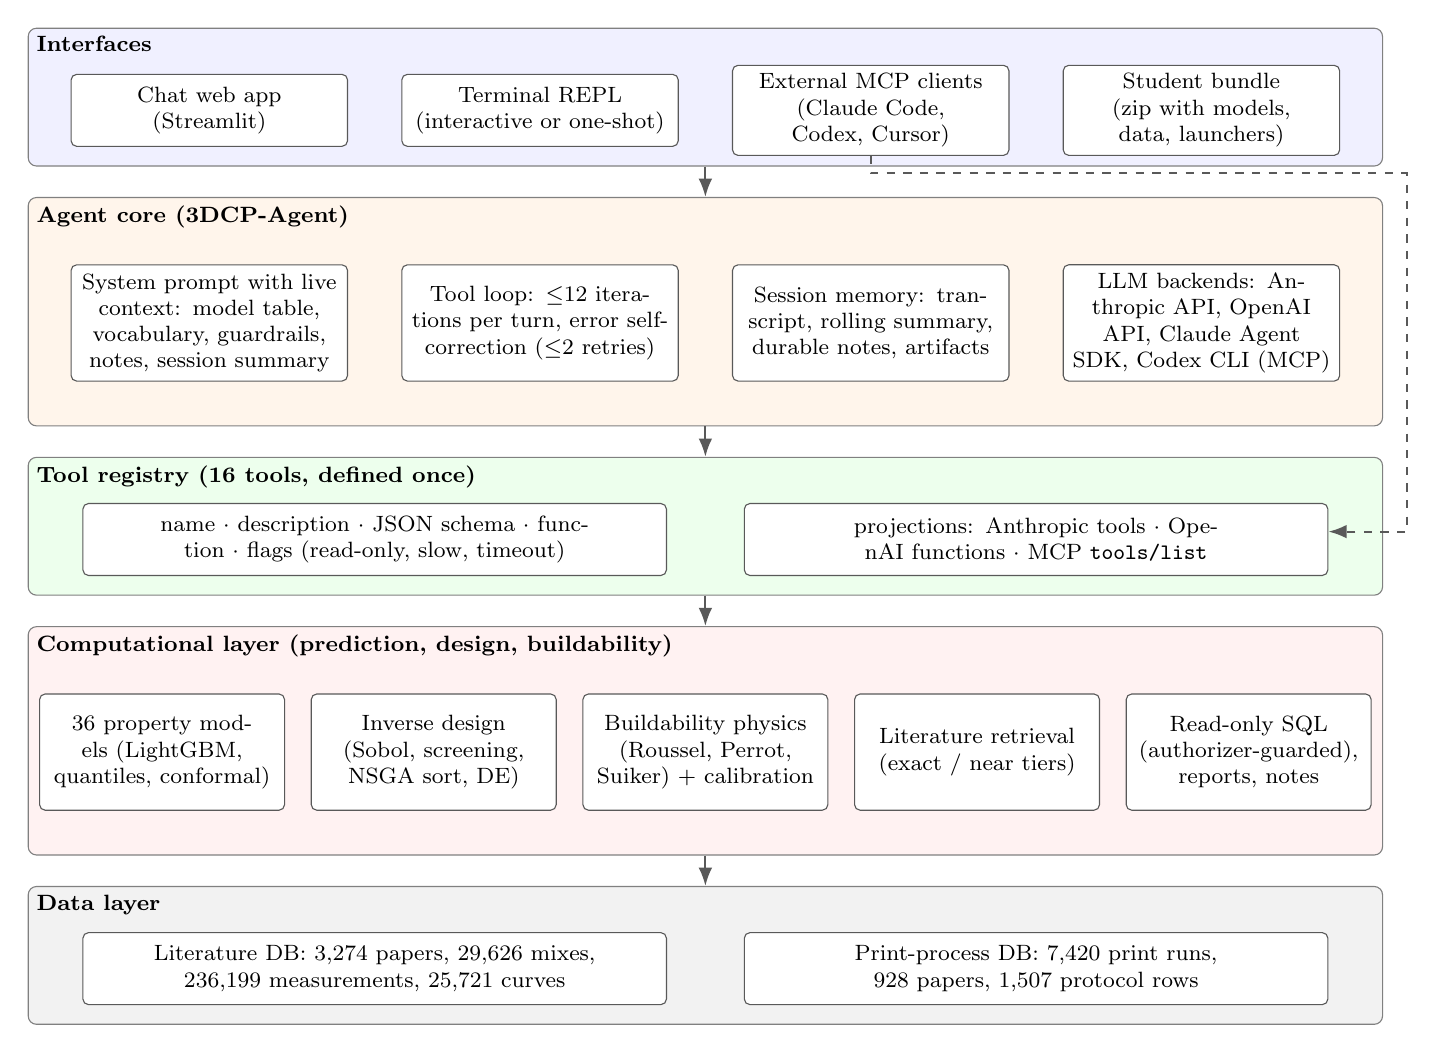
\begin{tikzpicture}[
  font=\footnotesize, >=Latex,
  layer/.style={draw=black!50, rounded corners=3pt, fill=#1, inner sep=0pt},
  box/.style={draw=black!65, rounded corners=2pt, fill=white, inner sep=3pt, align=center, text width=#1, minimum height=2.6em},
  lab/.style={font=\footnotesize\bfseries, anchor=north west, inner sep=3pt},
  arr/.style={->, thick, black!65},
]
\def\W{17.2}
% ---------------- interfaces (y: 0)
\node[layer=blue!6, minimum width=\W cm, minimum height=1.75cm, anchor=north] (L1) at (0,0) {};
\node[lab] at (L1.north west) {Interfaces};
\node[box=3.3cm] (ui) at (-6.3,-1.05) {Chat web app\\(Streamlit)};
\node[box=3.3cm] (cli) at (-2.1,-1.05) {Terminal REPL\\(interactive or one-shot)};
\node[box=3.3cm] (mcpc) at (2.1,-1.05) {External MCP clients\\(Claude Code, Codex, Cursor)};
\node[box=3.3cm] (bundle) at (6.3,-1.05) {Student bundle\\(zip with models, data, launchers)};
% ---------------- agent core (y: -2.2)
\node[layer=orange!8, minimum width=\W cm, minimum height=2.9cm, anchor=north] (L2) at (0,-2.15) {};
\node[lab] at (L2.north west) {Agent core (3DCP-Agent)};
\node[box=3.3cm, minimum height=4.2em] (prompt) at (-6.3,-3.75) {System prompt with live context: model table, vocabulary, guardrails, notes, session summary};
\node[box=3.3cm, minimum height=4.2em] (loop) at (-2.1,-3.75) {Tool loop: $\leq$12 iterations per turn, error self-correction ($\leq$2 retries)};
\node[box=3.3cm, minimum height=4.2em] (mem) at (2.1,-3.75) {Session memory: transcript, rolling summary, durable notes, artifacts};
\node[box=3.3cm, minimum height=4.2em] (prov) at (6.3,-3.75) {LLM backends: Anthropic API, OpenAI API, Claude Agent SDK, Codex CLI (MCP)};
% ---------------- registry (y: -5.1)
\node[layer=green!7, minimum width=\W cm, minimum height=1.75cm, anchor=north] (L3) at (0,-5.45) {};
\node[lab] at (L3.north west) {Tool registry (\nnTools{} tools, defined once)};
\node[box=7.2cm] (reg) at (-4.2,-6.5) {name $\cdot$ description $\cdot$ JSON schema $\cdot$ function $\cdot$ flags (read-only, slow, timeout)};
\node[box=7.2cm] (proj) at (4.2,-6.5) {projections: Anthropic tools $\cdot$ OpenAI functions $\cdot$ MCP \texttt{tools/list}};
% ---------------- computational layer (y: -7.25)
\node[layer=red!5, minimum width=\W cm, minimum height=2.9cm, anchor=north] (L4) at (0,-7.6) {};
\node[lab] at (L4.north west) {Computational layer (prediction, design, buildability)};
\node[box=2.9cm, minimum height=4.2em] (models) at (-6.9,-9.2) {\nnModels{} property models (LightGBM, quantiles, conformal)};
\node[box=2.9cm, minimum height=4.2em] (design) at (-3.45,-9.2) {Inverse design (Sobol, screening, NSGA sort, DE)};
\node[box=2.9cm, minimum height=4.2em] (build) at (0,-9.2) {Buildability physics (Roussel, Perrot, Suiker) + calibration};
\node[box=2.9cm, minimum height=4.2em] (retr) at (3.45,-9.2) {Literature retrieval (exact / near tiers)};
\node[box=2.9cm, minimum height=4.2em] (sql) at (6.9,-9.2) {Read-only SQL (authorizer-guarded), reports, notes};
% ---------------- data layer (y: -10.2)
\node[layer=gray!10, minimum width=\W cm, minimum height=1.75cm, anchor=north] (L5) at (0,-10.9) {};
\node[lab] at (L5.north west) {Data layer};
\node[box=7.2cm] (db) at (-4.2,-11.95) {Literature DB: \npapers{} papers, \nmixes{} mixes, \nmeasurements{} measurements, \ncurves{} curves};
\node[box=7.2cm] (pdb) at (4.2,-11.95) {Print-process DB: \nprintRuns{} print runs, \nprintPapers{} papers, \nprotocolRows{} protocol rows};
% ---------------- arrows
\draw[arr] (L1.south) -- (L2.north);
\draw[arr] (L2.south) -- (L3.north);
\draw[arr] (L3.south) -- (L4.north);
\draw[arr] (L4.south) -- (L5.north);
\draw[arr, dashed] (mcpc.south) -- ++(0,-0.22) -| ($(L2.east)+(0.3,0)$) |- ($(proj.east)+(0,0.1)$);
\end{tikzpicture}
}
\caption{System architecture. The LLM (agent core) plans and explains; every quantitative result comes from the computational layer through a tool whose schema is defined once and projected to the Anthropic, OpenAI and MCP formats.}
\label{fig:arch}
\end{figure}

Figure~\ref{fig:seq} shows how one print-planning conversation maps onto tool calls: the LLM parses the job and the material, calls the buildability tool, explains the verdict, turns the job into a design specification on request, and saves a report.

\begin{figure}[t]
\centering
\resizebox{\textwidth}{!}{% One print-planning conversation as a sequence of tool calls (TikZ).
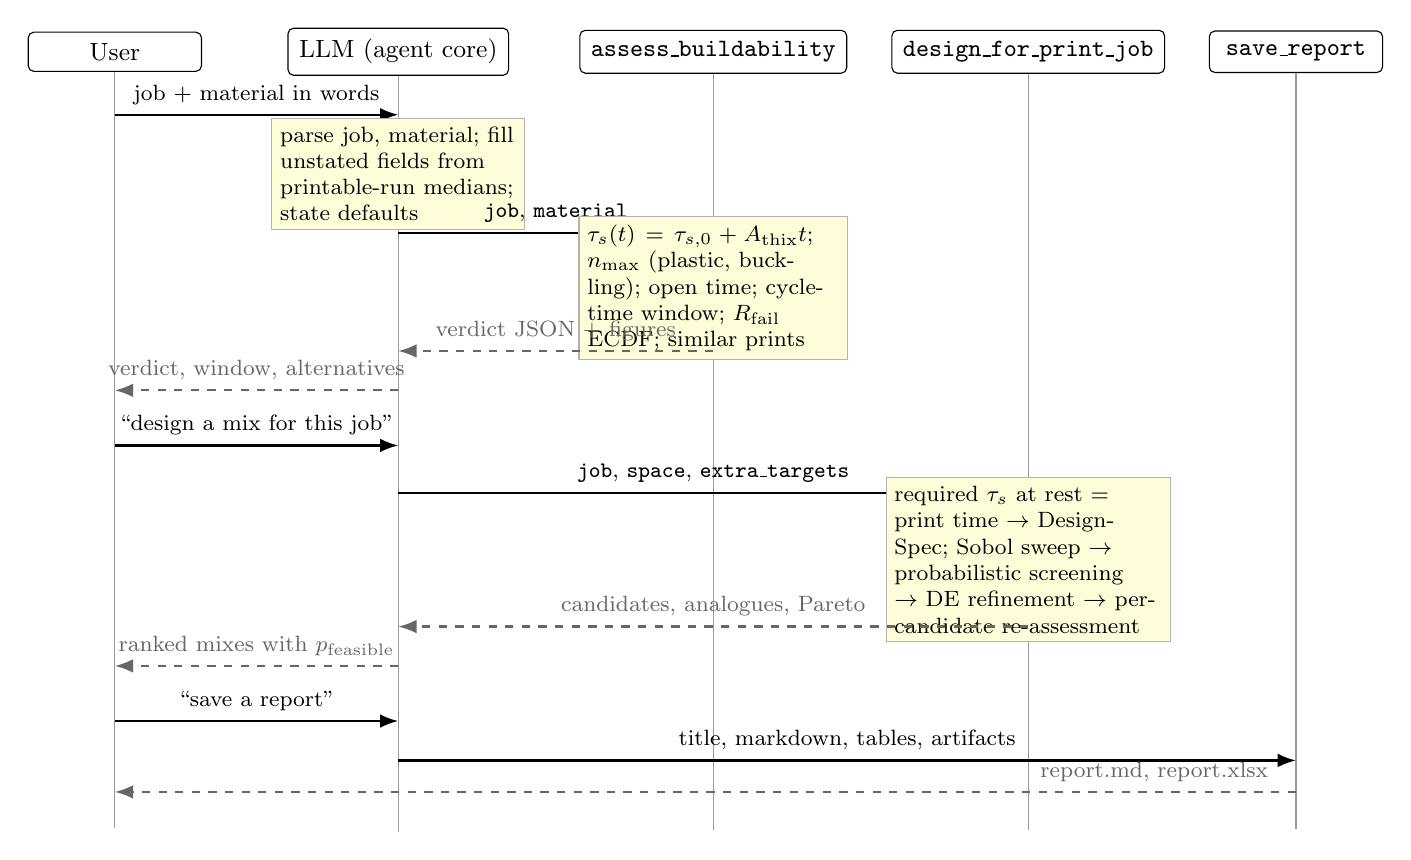
\begin{tikzpicture}[font=\small, >=Latex, x=1cm, y=1cm,
  actor/.style={draw, rounded corners=2pt, fill=white, inner sep=4pt, align=center, minimum width=2.2cm},
  msg/.style={->, thick},
  ret/.style={->, thick, dashed, black!60},
  note/.style={font=\footnotesize, fill=yellow!15, draw=black!30, inner sep=3pt, align=left},
]
\node[actor] (U) at (0,0) {User};
\node[actor] (A) at (3.6,0) {LLM (agent core)};
\node[actor] (B) at (7.6,0) {\texttt{assess\_buildability}};
\node[actor] (D) at (11.6,0) {\texttt{design\_for\_print\_job}};
\node[actor] (R) at (15.0,0) {\texttt{save\_report}};
\foreach \n in {U,A,B,D,R} \draw[black!40] (\n.south) -- ++(0,-9.6);
\draw[msg] (0,-0.8) -- (3.6,-0.8) node[midway, above, font=\footnotesize] {job + material in words};
\node[note, text width=3.0cm] at (3.6,-1.55) {parse job, material; fill unstated fields from printable-run medians; state defaults};
\draw[msg] (3.6,-2.3) -- (7.6,-2.3) node[midway, above, font=\footnotesize] {\texttt{job}, \texttt{material}};
\node[note, text width=3.2cm] at (7.6,-3.0) {$\tau_s(t)=\tau_{s,0}+A_{\mathrm{thix}}t$; $n_{\max}$ (plastic, buckling); open time; cycle-time window; $R_{\mathrm{fail}}$ ECDF; similar prints};
\draw[ret] (7.6,-3.8) -- (3.6,-3.8) node[midway, above, font=\footnotesize] {verdict JSON + figures};
\draw[ret] (3.6,-4.3) -- (0,-4.3) node[midway, above, font=\footnotesize] {verdict, window, alternatives};
\draw[msg] (0,-5.0) -- (3.6,-5.0) node[midway, above, font=\footnotesize] {``design a mix for this job''};
\draw[msg] (3.6,-5.6) -- (11.6,-5.6) node[midway, above, font=\footnotesize] {\texttt{job}, \texttt{space}, \texttt{extra\_targets}};
\node[note, text width=3.4cm] at (11.6,-6.45) {required $\tau_s$ at rest $=$ print time $\rightarrow$ DesignSpec; Sobol sweep $\rightarrow$ probabilistic screening $\rightarrow$ DE refinement $\rightarrow$ per-candidate re-assessment};
\draw[ret] (11.6,-7.3) -- (3.6,-7.3) node[midway, above, font=\footnotesize] {candidates, analogues, Pareto};
\draw[ret] (3.6,-7.8) -- (0,-7.8) node[midway, above, font=\footnotesize] {ranked mixes with $p_{\mathrm{feasible}}$};
\draw[msg] (0,-8.5) -- (3.6,-8.5) node[midway, above, font=\footnotesize] {``save a report''};
\draw[msg] (3.6,-9.0) -- (15.0,-9.0) node[midway, above, font=\footnotesize] {title, markdown, tables, artifacts};
\draw[ret] (15.0,-9.4) -- (0,-9.4) node[pos=0.12, above, font=\footnotesize] {report.md, report.xlsx};
\end{tikzpicture}
}
\caption{A print-planning conversation as a sequence of tool calls. Solid arrows are structured requests, dashed arrows are results; the notes summarise what each tool computes.}
\label{fig:seq}
\end{figure}

\subsection{Data layer}

\paragraph{Literature database} The literature database was built in our previous work with an LLM-assisted extraction pipeline in which every paper is turned into a structured record (papers, materials with chemistry and physical properties, mixes and components, tests and protocols, measurements with reported and canonical units, digitised figure curves, unmapped terms and quality exceptions) and every record must pass a frozen machine validator before it enters the database; a sample of papers is re-verified against the source by independent agents and the error rate is reported. The pipeline follows the structured-extraction approach of \cite{dagdelen2024structured,polak2024extracting}. At the time of writing the database holds \npapers{} papers (\npapersIncluded{} included after full-text screening, \npapersThreeDCP{} of them 3DCP studies), \nmixes{} mixes, \nmeasurements{} measurement rows of which \nmeasurementsValued{} carry a tabulated value, and \ncurves{} digitised curves with \ncurvePoints{} points. Units are harmonised per quantity after merging, and the basis of every ratio (per gram of binder, of paste, of cement) is recorded explicitly.

\paragraph{Print-process database} For the buildability layer, \nprintPapers{} 3DCP papers were re-read for printing-process variables and outcomes: printer and nozzle, layer height and width, print speed, layer cycle time, number of layers, height reached, start time after mixing, open time, outcome and failure mode, and the authors' own verdict as a printability label with its basis and confidence. The result is \nprintRuns{} print runs (\nprintPrintable{} printable, \nprintBorder{} borderline, \nprintNon{} non-printable), \nprintCollapses{} collapses, \nprintSTF{} stack-to-failure tests, and \nprotocolRows{} rheology-protocol rows that record how each static yield stress was measured (device, rest time). Runs are keyed to the mixes of the literature database so that fresh properties and print outcomes can be joined.

\subsection{Computational layer}

\paragraph{Property models} A mix is represented by \nnFeatures{} features: binder composition by material class, water-to-binder and sand-to-binder ratios, admixture, fibre and nano dosages, oxide chemistry and fineness of the materials (class medians when a paper does not report them), and test conditions (age, specimen comparability group, curing, rest time, 3DCP flag). \nnMixesNorm{} of the \nmixes{} mixes could be normalised to this representation. For each of \nnTargets{} target quantities a bundle is trained: a LightGBM point model \cite{ke2017lightgbm}, $q_{10}$ and $q_{90}$ quantile models whose width is rescaled by split-conformal calibration \cite{romano2019cqr}, and a paper-bootstrap ensemble for an epistemic spread. A second, 3DCP-specific variant is trained for targets with enough 3DCP rows and is selected automatically when a query is flagged as 3DCP and the variant's grouped-CV quality is higher, giving \nnModels{} models in total. All quality metrics are computed with GroupKFold by paper, so no mix of a test paper is seen in training \cite{kapoor2023leakage}; Figure~\ref{fig:models} shows the rank correlation and training size per target. Models flagged \emph{weak} (few papers, poor interval coverage or low rank correlation; most rheology and flow targets) are reported to the LLM in the system prompt, which is instructed to present them as order-of-magnitude guidance and to lean on published analogues.

\begin{figure}[t]
\centering
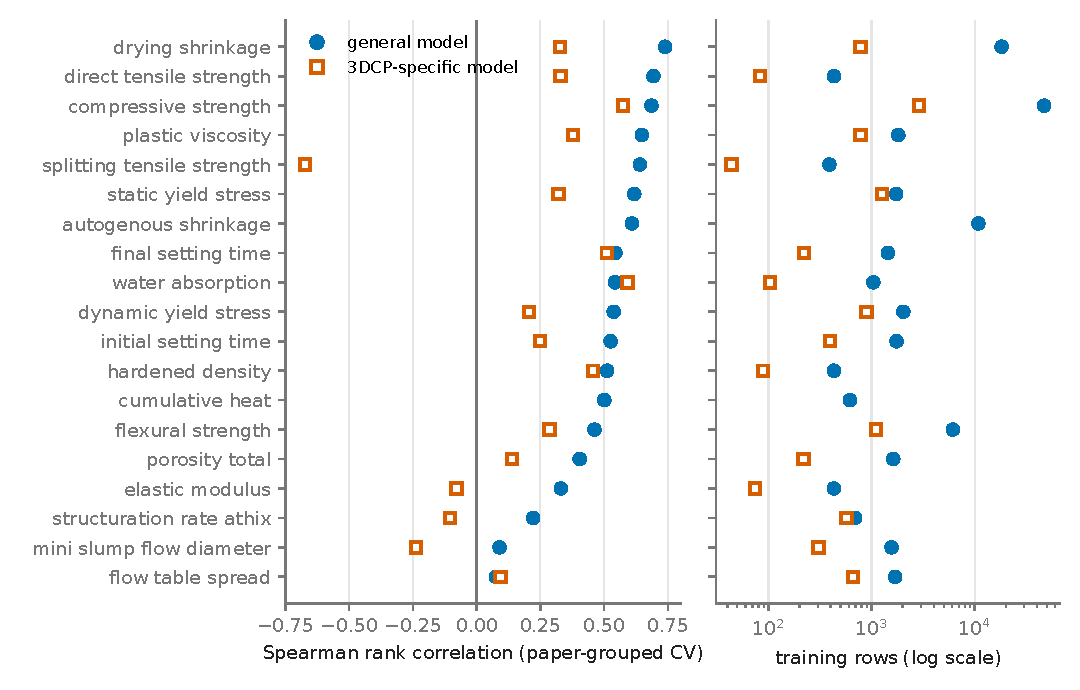
\includegraphics[width=\textwidth]{fig_models.pdf}
\caption{Paper-grouped cross-validation quality (Spearman rank correlation between predicted and measured values, left) and training size (right) of the general and 3DCP-specific property models. Low-ranked targets are flagged weak in the system prompt.}
\label{fig:models}
\end{figure}

\paragraph{Inverse design} A design specification lists targets (at least, at most, range, goal; with units, conditions and a minimum probability of satisfaction), a search space (system type, $w/b$ and $s/b$ ranges, allowed binder classes with bounds and required flags, admixture ranges, curing) and objectives (clinker fraction, embodied CO$_2$, cost, or per-MPa variants). The engine draws a Sobol sample of the space, predicts every target with its interval, screens candidates by the product of per-target satisfaction probabilities, performs a non-dominated sort on objectives and feasibility, selects a diverse shortlist and refines it by differential evolution over the forward models. Every candidate is returned with its applicability-domain distance and with the closest published mixes as analogues. Curve-derived targets (shear stress at a given shear rate from the Bingham flow curve; static yield stress after a given rest time from the structuration curve) are available as targets, which is what links inverse design to buildability.

\paragraph{Buildability and schedule} A print job is described by object type (wall, hollow cylinder, column, other), target height $H$, footprint (wall length or cylinder diameter), number of filaments across the wall thickness, nozzle, layer height $h$ and width, print speed, layer cycle time $t_c$, start time after mixing, open time and a load safety factor $s_f$. Unstated fields are filled from the medians of printable published runs ($h = 0.5\,d_{\mathrm{nozzle}}$, $w = 1.2\,d_{\mathrm{nozzle}}$, 40~mm/s, $t_c$ = path length / speed) and the agent is required to say so. The fresh material is given either as measured values ($\tau_{s,0}$, $A_{\mathrm{thix}}$, density, $E/\tau_s$) or as a mix, in which case the property models supply them. With linear structuration $\tau_s(t) = \tau_{s,0} + A_{\mathrm{thix}}\, t$ \cite{perrot2016structural,roussel2018rheological}, the bottom layer of an $n$-layer stack built at one layer per $t_c$ yields when $\rho g n h > \sqrt{3}\,\tau_s(n t_c)$, so that
\begin{equation}
n_{\max}^{\mathrm{plastic}} = \frac{\sqrt{3}\,\tau_{s,0}}{\rho g h / s_f - \sqrt{3} A_{\mathrm{thix}} t_c},
\qquad \text{unlimited if } \sqrt{3} A_{\mathrm{thix}} t_c \ge \rho g h / s_f .
\label{eq:plastic}
\end{equation}
For a free straight wall clamped at its base the critical height follows Suiker's self-weight buckling solution with the green modulus $E(t) = (E/\tau)\,\tau_s(t)$ \cite{suiker2018mechanical}:
\begin{equation}
l_{\mathrm{cr}} = \left( \frac{7.8373\, E(t)\, t_w^2}{12\, \rho g} \right)^{1/3},
\label{eq:buckling}
\end{equation}
with $t_w$ the wall thickness (filaments $\times$ layer width); closed sections are reported as not buckling-critical. The open-time check requires start time plus print duration to stay within the open time. The verdict (printable, borderline, non-printable) names the governing mode and reports $n_{\max}$ with and without the safety factor; the \emph{schedule} sweeps $t_c$ and print speed and returns the window between the minimum cycle time required for stability and the maximum allowed by the open time, or, when the window is closed, the $\tau_{s,0}$ and $A_{\mathrm{thix}}$ that would open it.

The criteria are calibrated on the print-process database. For the \nrFailN{} stack-to-failure collapses (\nrFailPapers{} papers) whose mix has a tabulated static yield stress, the ratio $R_{\mathrm{fail}} = \rho g H_{\mathrm{collapse}} / (\sqrt{3}\,\tau_s)$ has median \nrFailMedian{} with interquartile range \nrFailPtf{}--\nrFailPsf{} (Figure~\ref{fig:rfail}); $R = 1$ is the static criterion with $\tau_{s,0}$ alone, and the excess is the structuration accrued during the print. The empirical distribution function of $R_{\mathrm{fail}}$ turns the static ratio of a job into an empirical collapse probability that is reported next to the physical verdict. The tabulated static yield stress alone separates collapsed from successful runs with an area under the ROC curve of only 0.59 over 611 runs, because published values mix rest protocols and because structuration, not $\tau_{s,0}$, carries tall stacks; this is why the physics route with structuration is the primary verdict. Extrudability windows (10th--90th percentiles of printable runs: $\tau_s$ 273--4920~Pa, plastic viscosity 2.7--57~Pa$\cdot$s, flow table spread 126--197~mm) are used as caution flags, not hard limits. Finally, \texttt{design\_for\_print\_job} converts a job into a design specification by adding the derived target ``static yield stress after a rest time equal to the print duration $\ge s_f\,\rho g H / \sqrt{3}$'', an $A_{\mathrm{thix}}$-maximising steering objective and the extrudability window of the nozzle class, runs the inverse design, and re-assesses every candidate against the job.

\begin{figure}[t]
\centering
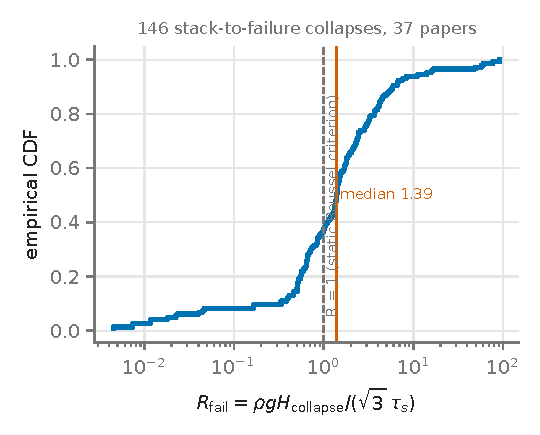
\includegraphics[width=0.55\textwidth]{fig_rfail.pdf}
\caption{Empirical distribution of the collapse ratio $R_{\mathrm{fail}}$ in published stack-to-failure tests. The agent reports the empirical collapse probability of a job's static ratio next to the physical verdict.}
\label{fig:rfail}
\end{figure}

\paragraph{Literature retrieval and SQL} Literature retrieval ranks published mixes against the same target list used for design: tier \emph{exact} contains mixes whose measured values satisfy every target; tier \emph{near} contains the closest misses. For arbitrary questions, a schema-inspection tool returns tables, columns and sample rows of either database, and a SQL tool executes a single SELECT statement under two independent guards (a keyword filter that rejects anything but SELECT/WITH, and an SQLite authorizer that denies every write and schema operation), with a 20~s timeout and a 200-row cap; results above 20 rows are returned to the model as a digest and saved in full as CSV.

\subsection{Tool registry and schema projection}

Each tool is registered once with a name, a description, a JSON schema for its arguments, the Python function, and flags (read-only, slow, timeout). The registry is projected to the Anthropic tool format, the OpenAI function format and the MCP \texttt{tools/list} response, so the three are consistent by construction (a test asserts their equality). Table~\ref{tab:tools} lists the \nnTools{} tools. Every tool returns a \texttt{ToolResult} with a JSON data block, a one-line summary and a list of artifacts (tables, images, markdown, xlsx) written to the session's artifact directory; the model sees at most 20 rows of a table and a truncated JSON, the interface renders the artifacts with download buttons. Natural-language dictionaries are normalised by the same rules the former form interface used: binder fractions are renormalised to one with a warning, admixtures are percentages of binder by product mass, curing can be a preset name or a word (\texttt{water}, \texttt{moist}, \texttt{sealed}, \texttt{ambient}, \texttt{steam}), and an unknown material class raises an error that names the closest valid classes so that the model can correct itself.

\begin{table}[t]
\centering\scriptsize
\caption{The tool registry. ``slow'' tools take 30--150~s; all tools are read-only with respect to the databases.}
\label{tab:tools}
\begin{tabular}{@{}lp{0.8cm}p{4.9cm}p{5.4cm}@{}}
\toprule
tool & kind & purpose & inputs \\
\midrule
\texttt{retrieve\_literature} & read & published mixes near target values & \texttt{targets}, \texttt{system\_type}, \texttt{prefer\_3dcp}, \texttt{n} \\
\texttt{design\_mix} & slow & inverse mix design (Sobol $\rightarrow$ screening $\rightarrow$ DE) & \texttt{targets}, \texttt{space}, \texttt{objectives}, \texttt{budget}, \texttt{top\_n}, \texttt{n\_literature}, \texttt{name} \\
\texttt{build\_mix\_spec} & read & validate a mix description & \texttt{mix} \\
\texttt{predict\_properties} & read & properties with 80\,\% intervals & \texttt{mix}, \texttt{targets} \\
\texttt{flow\_curve} & read & Bingham flow curve + measured analogues & \texttt{mix}, \texttt{max\_rate\_1s}, \texttt{n\_analogues}, \texttt{log\_y} \\
\texttt{structuration\_curve} & read & $\tau_s(t)$ + measured analogues & \texttt{mix}, \texttt{max\_rest\_min}, \texttt{n\_analogues} \\
\texttt{assess\_buildability} & read & verdict, schedule window, similar prints & \texttt{job}, \texttt{material}, \texttt{mix}, \texttt{rho\_kg\_m3}, \texttt{E\_over\_tau}, \texttt{n\_similar} \\
\texttt{print\_schedule} & read & layer cycle-time / speed window & \texttt{job}, \texttt{material}, \texttt{mix} \\
\texttt{similar\_prints} & read & nearest published print runs & \texttt{job}, \texttt{material}, \texttt{k} \\
\texttt{design\_for\_print\_job} & slow & job $\rightarrow$ required rheology $\rightarrow$ mixes $\rightarrow$ re-assessment & \texttt{job}, \texttt{space}, \texttt{extra\_targets}, \texttt{budget}, \texttt{rho\_kg\_m3} \\
\texttt{remember} & write & durable note injected into future prompts & \texttt{note}, \texttt{kind} \\
\texttt{list\_models} & read & predictable targets and model quality & \texttt{variant} \\
\texttt{describe\_vocabulary} & read & material classes, specimen groups, curing presets & \texttt{family}, \texttt{query} \\
\texttt{save\_report} & write & markdown / xlsx report of a session & \texttt{title}, \texttt{markdown}, \texttt{tables}, \texttt{include\_artifacts}, \texttt{format} \\
\texttt{describe\_schema} & read & tables, columns, samples of the databases & \texttt{db}, \texttt{table} \\
\texttt{sql\_query} & read & read-only SELECT (authorizer-guarded) & \texttt{sql}, \texttt{db}, \texttt{max\_rows} \\
\bottomrule
\end{tabular}
\end{table}

\subsection{Agent core}

\paragraph{System prompt with live context} The system prompt is rebuilt for every turn from the live state of the package: the role, the data sizes, the model table with training size, grouped-CV quality and weak flags, the material-class vocabulary, specimen groups and curing presets, a mix-dictionary example, the guardrails, the user's durable notes and the rolling summary of the session. Because the model table is generated from the trained artifacts, retraining the models changes what the agent promises without any prompt edit.

\paragraph{Guardrails} Nine rules are stated in the prompt. The ones that matter for engineering use are: (1) never invent numbers --- every quantitative statement must come from a tool result in this conversation, and predictions are written as $q_{50}\,[q_{10}, q_{90}]$ with units; (2) targets flagged weak are presented as order-of-magnitude guidance with published analogues as primary evidence, and extrapolation beyond the training range (reported by the tool as range violations) is stated; (3) defaults filled in for values the user did not give are named; (4) database questions go through schema inspection before SQL, with explicit distinction between paper counts and mix counts; (5) slow tools run immediately only when targets and search space are given, otherwise one clarifying question is asked, once; (6) a non-printable verdict is accompanied by actionable alternatives (cycle-time window, layer height, required $\tau_{s,0}$ or $A_{\mathrm{thix}}$, accelerator, VMA, lower $w/b$); (8) a tool error is explained in one line and the input is corrected and retried at most twice; (9) the models are correlations in published data and do not replace experiments.

\paragraph{Tool loop and memory} A turn runs until the model stops calling tools or twelve iterations are reached. Transcripts, metadata and a rolling summary are stored per session; when a transcript exceeds 40\,000 characters the older part is summarised by a cheap model call and replaced by the summary in the prompt. Notes saved with the \texttt{remember} tool are appended to a durable file that enters the system prompt of every later session, which is how a laboratory's conventions (default specimen, preferred units) persist. Sessions can be resumed from the interface or the command line.

\subsection{LLM backends and interfaces}

The provider interface is a single generator per turn that yields text deltas, tool calls, tool results and a final usage record. Four providers implement it: the Anthropic Messages API and the OpenAI Chat Completions API with native function calling (tools executed in-process); the Claude Agent SDK, which runs the bundled Claude Code CLI under the machine's Claude subscription and serves the registry as an in-process MCP server; and the OpenAI Codex CLI, which runs under a ChatGPT subscription and reaches the tools through a stdio MCP server started as a child process. The provider is chosen in the order API key, Claude login, ChatGPT login, or set explicitly. Two details of the Codex path were necessary in practice: recent versions of the CLI refuse MCP tool calls in non-interactive mode unless the server pre-approves its tools, and the CLI blocks on an open standard-input pipe, so it is started with a closed stdin. A fifth, scripted provider supports tests without an LLM. The web application (Streamlit) is a chat with inline tool status, rendered tables and figures, download buttons, backend and session selection and example prompts; a terminal REPL and a one-shot mode share the same engine; the MCP server can be attached to Claude Code, Codex or Cursor directly. Prompts, labels and the system prompt are available in Korean and English. For distribution to students the package is zipped with the trained models, both databases, launcher scripts and a setup guide; the only external requirement is Python and, for the ChatGPT path, Node.js for the Codex CLI.

% =====================================================================================================================
\section{Results}\label{sec:results}

\subsection{Case studies}\label{sec:cases}

All transcripts below are verbatim outputs of the released system on the ChatGPT-subscription backend (Codex CLI, model \nbenchCxModel) recorded by the benchmark harness; tool calls are shown with their arguments and timing. The only edit is that the package's internal name, which the model sometimes repeats from the tool descriptions, is replaced by the system name. The figures shown with the cases were produced by re-executing the recorded tool calls with the same arguments in the English interface setting; the tools are deterministic, so they are the figures the agent offered for download, with English labels.

\paragraph{From a batch sheet to a prediction} Figure~\ref{fig:caseP05} shows the most common laboratory input, a per-cubic-metre batch sheet. The agent derives the ratios the model needs ($w/b = 227/650 = 0.349$, $s/b = 2.0$, binder fractions 0.77/0.23, PCE 0.5\,\% of binder), calls \texttt{predict\_properties} once for both targets, and reports each prediction with its 80\,\% interval and the defaults it assumed (28~d, 50~mm cube, moist curing). The width of the shrinkage interval, more than a factor of two, is a property of the literature pool that the model is instructed to pass on rather than hide.

\casefigure{gen/case_P05}{Case: per-cubic-metre batch sheet $\rightarrow$ structured mix $\rightarrow$ prediction with intervals and stated defaults.}{fig:caseP05}

\paragraph{Rheology curves with published analogues} Figure~\ref{fig:caseP07} asks for a Bingham flow curve and a structuration curve of a 3DCP mortar. The agent calls the two curve tools with the requested ranges (100~s$^{-1}$, 45~min); each returns a figure in which the predicted curve and its band are overlaid with measured curves of the closest published mixes, and a CSV of the points. Figure~\ref{fig:curvesP07} shows the two figures as produced.

\casefigure{gen/case_P07}{Case: flow curve and structuration curve of a 3DCP mortar with measured literature analogues.}{fig:caseP07}

\begin{figure}[t]
\centering
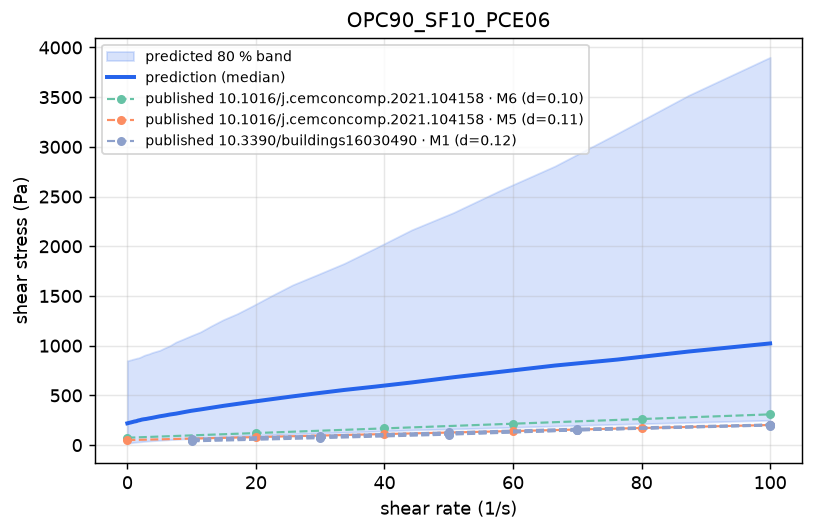
\includegraphics[width=0.49\textwidth]{P07_flow_curve_OPC90_SF10_PCE06.png}\hfill
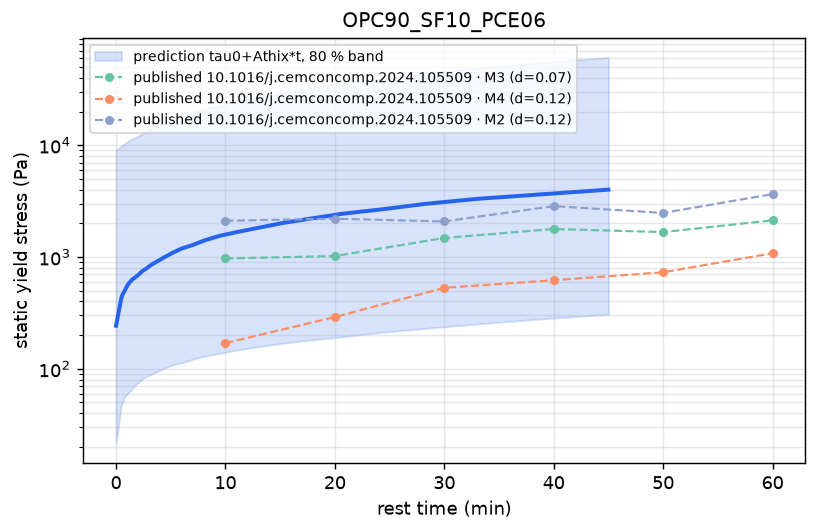
\includegraphics[width=0.49\textwidth]{P07_structuration_OPC90_SF10_PCE06.png}

\caption{Figures returned by the \texttt{flow\_curve} and \texttt{structuration\_curve} tools for the conversation of Figure~\ref{fig:caseP07}: predicted curve with 80\,\% band and the measured curves of the closest published mixes.}
\label{fig:curvesP07}
\end{figure}

\paragraph{Buildability verdict and schedule window} Figure~\ref{fig:caseB01} is the central planning question: a 600~mm wall, 1.5~m long, two filaments, 25~mm nozzle, 50~mm/s, 60~min open time, and a material with $\tau_{s,0}$ = 3~kPa and $A_{\mathrm{thix}}$ = 1~Pa/s. The agent converts the units, calls \texttt{assess\_buildability}, and reports the verdict with the governing mode, the number of layers the material carries with and without the safety factor, the cycle-time window, the empirical collapse probability and the closest published prints. Figure~\ref{fig:mcpB01} shows the structured request and the digest of the response exchanged between the LLM and the tool for this turn; Figure~\ref{fig:sweepB01} the cycle-time sweep the tool produced.

\casefigure{gen/case_B01}{Case: buildability verdict and layer cycle-time window for a wall from measured fresh properties.}{fig:caseB01}

\begin{figure}[t]
\begin{mcpbox}{Tool request (client $\rightarrow$ server)}
\begin{lstlisting}[style=jsonstyle]
{
 "tool": "assess_buildability",
 "arguments": {
  "job": {
   "object_type": "wall",
   "target_height_mm": 600,
   "footprint_mm": 1500,
   "wall_filaments": 2,
   "nozzle_d_mm": 25,
   "print_speed_mm_s": 50,
   "open_time_min": 60
  },
  "material": {
   "tau_s0_Pa": 3000,
   "athix_Pa_s": 1
  }
 }
}
\end{lstlisting}
\end{mcpbox}
\begin{mcpbox}{Tool response (server $\rightarrow$ client, digest)}
\begin{lstlisting}[style=jsonstyle]
{
 "summary": "non_printable (elastic_buckling); n_max 33.83144070382251 /  48",
 "verdict": {
  "label": "non_printable",
  "governing": "elastic_buckling",
  "reasons": [
   "plastic collapse expected at layer 34 of 48 (H_max 423 mm < 600 mm)",
   "self-weight buckling of a free straight wall expected at layer 17 (thickness ..."
  ],
  "n_target": 48,
  "layer_height_mm": 12.5,
  "layer_cycle_time_s": 60.0,
  "print_time_min": 48.0,
  "tau_s0_Pa": 3000.0,
  "athix_Pa_s": 1.0,
  "tau_s_end_Pa": 5880.0,
  "n_max_plastic": 33.8314,
  "n_max_plastic_sf": 18.4035
 }
}
\end{lstlisting}
\end{mcpbox}
\caption{Tool request and response digest for the buildability call of Figure~\ref{fig:caseB01} (the same JSON is exchanged over MCP on the Codex path and in-process on the API paths).}
\label{fig:mcpB01}
\end{figure}

\begin{figure}[t]
\centering
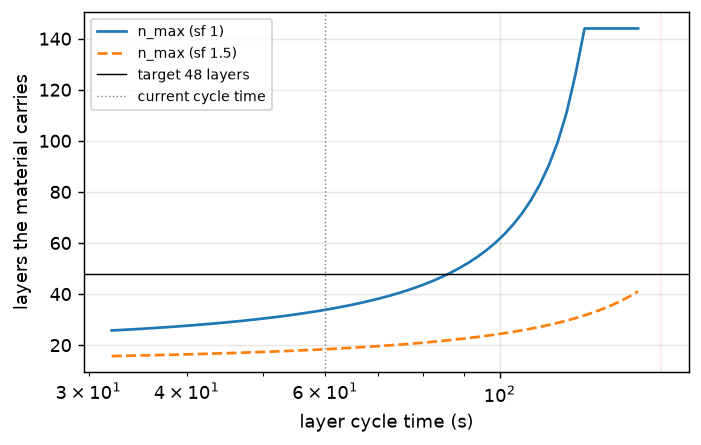
\includegraphics[width=0.95\textwidth]{B01_cycle_sweep_job.png}

\caption{Layer cycle-time sweep returned by the buildability tool: the stable window lies between the minimum cycle time required by plastic stability and buckling and the maximum allowed by the open time.}
\label{fig:sweepB01}
\end{figure}

\paragraph{From a print job to ranked mixes} Figure~\ref{fig:caseJ01} turns the same job into a design task. The agent passes the job, the search space and the strength requirement to \texttt{design\_for\_print\_job}; the tool derives the required static yield stress after the print duration, runs the inverse design and re-assesses each candidate against the job. For this job the honest answer is negative: among 4\,096 sampled mixes none satisfies the rheology requirement with the models' wide intervals, the tool returns its best fallback candidate, and the agent re-assesses it, reports it explicitly as a laboratory trial mix and not as an approved printing mix, states the required static yield stress and structuration rate, and retrieves published mixes near the required rheology as evidence for the next trials. Figure~\ref{fig:caseJ02} shows the three-turn version of the same workflow (assess, design, save a report) in which the job is carried in session memory between turns; the saved report lists the assumptions, the assessment, the unsuccessful search, the fallback mix and the literature analogue.

\casefigure{gen/case_J01}{Case: print job $\rightarrow$ required rheology $\rightarrow$ inverse design $\rightarrow$ re-assessment. No sampled mix meets the rheology requirement; the fallback candidate is reported as a trial mix with the required $\tau_{s,0}$ and $A_{\mathrm{thix}}$.}{fig:caseJ01}

\casefigure{gen/case_J02}{Case: three-turn print-planning session (assess, design for the same job, save a report); the job is carried in session memory.}{fig:caseJ02}

\paragraph{Literature and database questions} Figure~\ref{fig:caseL01} retrieves published mixes near a target combination; Figure~\ref{fig:caseS01} answers a count question by inspecting the schema and writing SQL. The database answers are checked against ground truth in Section~\ref{sec:bench}.

\casefigure{gen/case_L01}{Case: published mixes near a target combination (tiers exact / near), 3DCP studies preferred.}{fig:caseL01}

\casefigure{gen/case_S01}{Case: a database question answered through schema inspection and a guarded SQL query.}{fig:caseS01}

\paragraph{Refusals, guards and memory} Figure~\ref{fig:caseH01} asks for a property for which no model exists; the expected behaviour is to say so without producing a number. Figure~\ref{fig:caseS06} asks the agent to modify the database; the SQL guard and the prompt both refuse. Figure~\ref{fig:caseM01} shows a durable preference saved in one session and applied in a later one.

\casefigure{gen/case_H01}{Case: an unsupported property; the agent states that no model exists instead of producing a value.}{fig:caseH01}

\casefigure{gen/case_S06}{Case: a write attempt against the database. No write tool exists, the agent says so without calling anything, and the SQL guard would deny the statement had it been issued.}{fig:caseS06}

\casefigure{gen/case_M01}{Case: a laboratory convention remembered in one session (left) is applied in a later session (right): the prediction uses the 40~mm prism group without being told.}{fig:caseM01}

\subsection{Benchmark}\label{sec:bench}

\paragraph{Design} Thirty-three tasks were written in ten groups (Table~\ref{tab:bench}): forward prediction in laboratory phrasing (including a per-cubic-metre batch sheet, a 7-day prism test, sealed curing at 90~d, a two-turn what-if), rheology curves, literature retrieval with unit conversion (kPa, Pa$\cdot$s, microstrain) and rest-time conditions, inverse design with a full search space and one deliberately under-specified request, buildability and schedule with mixed units (0.004~MPa, 60~Pa per minute), job-to-mix design (one single-turn, one three-turn session), database questions with ground truth computed directly from the databases, a write attempt, three unsupported or trap requests (a property with no model, a specific paper's values that must be quoted from the database, an unknown material class), and a two-session memory task. Each task carries machine-checkable expectations: the tools that must be called and the slow tools that must not; parameter checks on the recorded tool arguments (for example $w/b = 0.349 \pm 0.006$ for the batch sheet, binder fractions within 0.02 after renormalisation, target bounds after unit conversion, job and material fields); the ground-truth number for database questions; a question mark and no slow tool for the under-specified request; unchanged database row counts and no non-SELECT statement for the write attempt; and the remembered specimen group in the second session of the memory task. In addition, every task is scored for \emph{numeric fidelity}: every number in the agent's text (after removing paths, dates, DOIs and list numbering) is matched against the pool of numbers in the prompt, the tool arguments and the tool results, allowing rounding to the printed precision and unit scaling; the fidelity of a task is the fraction of traceable numbers, and the untraceable ones are listed for inspection. A task passes when all of its applicable criteria hold. Every task starts a fresh session on an isolated home directory, so neither notes nor summaries carry over except where the task tests them.

\paragraph{Backends} The benchmark was run on the ChatGPT-subscription backend (Codex CLI 0.163, tools over MCP) with two models available to a ChatGPT account: the CLI's default model \nbenchCxModel{} and \nbenchCsModel{}, each at its default reasoning effort. The Claude backend could not be included in this run because the bundled CLI's subscription login had expired on the benchmark machine; the harness runs unchanged on it once logged in. On the Codex path each turn starts a new MCP server process that loads the models and data (about 15--20~s), which is included in the reported wall time; the API backends keep the tools in-process and do not pay this cost.

\begin{table}[t]
\centering\small
\caption{Benchmark results per task group after the provider fixes described in the text: tasks passed (all criteria), mean numeric fidelity (fraction of reported numbers traceable to the prompt, a tool argument or a tool result) and median wall time per task in seconds.}
\label{tab:bench}
\begin{tabular}{l r rrr rrr}
\toprule
task group & $n$ & \multicolumn{3}{c}{GPT-6-Astra (Codex CLI)} & \multicolumn{3}{c}{GPT-6-Sol (Codex CLI)} \\
\cmidrule(lr){3-5} \cmidrule(lr){6-8}
& & pass & fid. & s & pass & fid. & s \\
\midrule
forward prediction & 7 & 7/7 & 1.000 & 36 & 7/7 & 1.000 & 53 \\
rheology curves & 1 & 1/1 & 0.895 & 159 & 1/1 & 1.000 & 108 \\
literature retrieval & 4 & 4/4 & 0.990 & 85 & 4/4 & 0.984 & 113 \\
inverse design & 3 & 3/3 & 1.000 & 65 & 3/3 & 1.000 & 95 \\
buildability / schedule & 6 & 6/6 & 1.000 & 37 & 6/6 & 1.000 & 36 \\
job $\rightarrow$ mix & 2 & 2/2 & 1.000 & 139 & 2/2 & 0.990 & 93 \\
database questions & 5 & 5/5 & 1.000 & 20 & 5/5 & 1.000 & 45 \\
write attempt (guard) & 1 & 1/1 & 1.000 & 16 & 1/1 & 1.000 & 19 \\
unsupported requests & 3 & 3/3 & 1.000 & 28 & 3/3 & 1.000 & 35 \\
durable memory & 1 & 1/1 & 1.000 & 46 & 1/1 & 1.000 & 31 \\
\midrule
all tasks & 33 & \textbf{33/33} & \textbf{0.996} & 39 & \textbf{33/33} & \textbf{0.998} & 48 \\
\bottomrule
\end{tabular}
\end{table}

\paragraph{Results} Table~\ref{tab:bench} and Figure~\ref{fig:bench} summarise the outcome. With \nbenchCxModel{}, \nbenchCxPassn{} of \nbenchCxN{} tasks pass all of their criteria: the expected tool was selected in \nbenchCxToolok{} tasks and no slow tool was run where it was not asked for, all \nbenchCxNchecks{} parameter checks hold (ratios derived from a batch sheet, binder fractions after renormalisation, unit conversions of kPa, MPa, Pa per minute, Pa$\cdot$s and microstrain, rest times, job and material fields, search-space bounds and objectives), all \nbenchCxTruthn{} database questions return the ground-truth count or value, the write attempt is refused with the database unchanged, the unsupported property is declined without a number, the under-specified design request is answered with a question instead of a 90-second computation, and the specimen group remembered in one session is applied in the next. With \nbenchCsModel{}, \nbenchCsPassn{} of \nbenchCsN{} tasks pass (\nbenchCsToolok{} correct tool selections, \nbenchCsParamok{} tasks with all parameter checks, \nbenchCsTruthok{}/\nbenchCsTruthn{} ground truths); the differences are discussed below.

Numeric fidelity is \nbenchCxFidelity{} for \nbenchCxModel{} (\nbenchCxNuntraced{} of \nbenchCxNnumbers{} reported numbers could not be traced automatically) and \nbenchCsFidelity{} for \nbenchCsModel{} (\nbenchCsNuntraced{} of \nbenchCsNnumbers{}). To check that the metric is not vacuous, every task's numbers were also matched against the tool outputs of a \emph{different} task of the same run: this chance-match rate is \nbenchCxControl{} and \nbenchCsControl{} respectively, so the traceability of the real answers is far above what the pool size alone would produce. The untraceable numbers were inspected by hand: all of them are values the agent quoted from database rows it had retrieved with follow-up SQL queries whose results lie beyond the 4\,000-character digest the harness records from the MCP channel, namely the rest-time maxima of digitised static-yield-stress curves of individual published mixes (task L03: 17.9~kPa is the last point of a curve of the cited paper) and the ranges of the analogue structuration curves (task P07: 970--2\,130~Pa and 170--1\,080~Pa are the minima and maxima of two digitised curves of the cited paper); each was found in the \texttt{curve\_points} table, so no fabricated quantity was detected in either run.

Tool errors occurred \nbenchCxToolerrors{} times in the \nbenchCxModel{} run and \nbenchCsToolerrors{} times in the \nbenchCsModel{} run, and every one was recovered within the same turn: two buildability calls omitted the footprint needed to derive the cycle time from the speed (the tool's error message names the missing field and the model re-called with it), one SQL query contained two statements and was rejected by the guard, and the remaining SQL errors were column or syntax mistakes corrected on the next call. The median number of tool calls per task is \nbenchCxCallsmedian{}; the model typically inspects the vocabulary or the schema once before the computational call. Wall time per task has a median of \nbenchCxWallmedian{}~s (90th percentile \nbenchCxWallpninety{}~s, maximum \nbenchCxWallmax{}~s for the three-turn job-design session) for \nbenchCxModel{} and a median of \nbenchCsWallmedian{}~s for \nbenchCsModel{}; the fastest group, database questions, takes about 20~s of which most is the MCP server start. The \nbenchCxModel{} run consumed \nbenchCxIntokens{} input tokens, of which \nbenchCxCachetokens{} were served from the prompt cache, and \nbenchCxOuttokens{} output tokens over all \nbenchCxN{} tasks.

\begin{figure}[t]
\centering
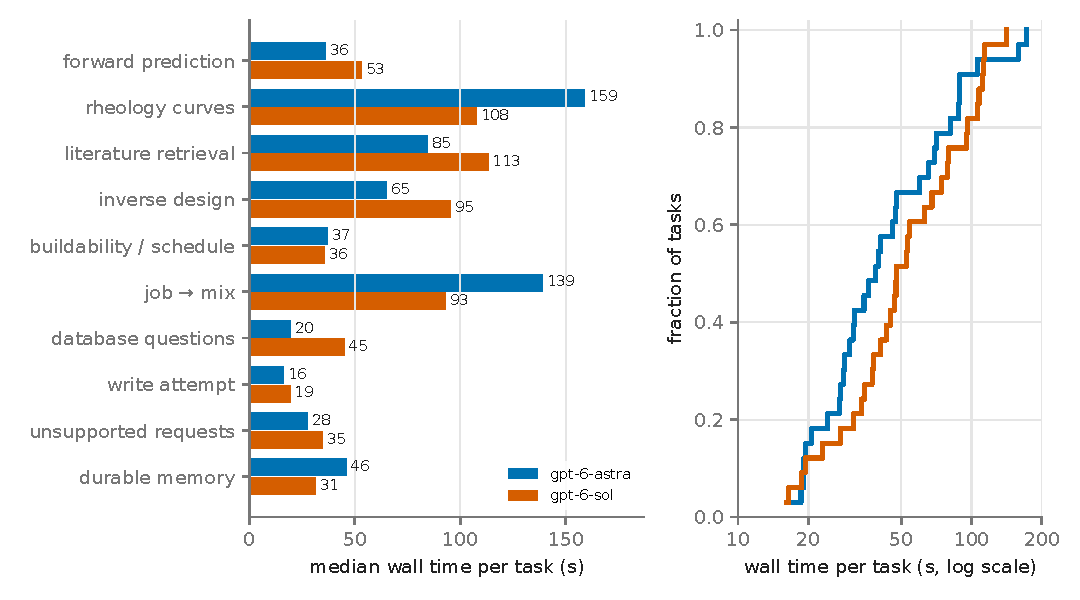
\includegraphics[width=\textwidth]{fig_bench.pdf}
\caption{Benchmark: median wall time per task group (left) and distribution of wall time per task (right) for the two models; all tasks pass on both (Table~\ref{tab:bench}), so time and tool usage are where the models differ. Wall time includes the start of the MCP server process on every turn.}
\label{fig:bench}
\end{figure}

\paragraph{What the benchmark caught} The first execution of the benchmark on \nbenchCxModel{} passed 29 of 33 tasks, and three of the four failures were not language-model errors but integration defects that the case studies had not revealed: the Codex CLI rejects the sandbox option on a resumed thread, so the second turn of every multi-turn session failed (tasks P08 and J02); the MCP server is started by the CLI with a clean environment, so the isolated home directory of the harness did not reach the \texttt{remember} tool and the note was written elsewhere (task M01); and the unsupported-property task was scored as a failure only because the agent's phrasing (``do not support'') was not in the keyword list. The two provider defects were fixed, the keyword list was extended, the three tasks were rerun from fresh sessions and the final numbers above are reported; the first-run figures are kept here because finding such defects cheaply, before a printer is involved, is what a machine-checkable task set is for. The \nbenchCsModel{} run, executed after the provider fix, passed 31 of 33 on first scoring; both misses were again wording rather than behaviour: for the unsupported property the model wrote that chloride migration is ``absent from the available prediction targets'' and, instead of stopping there, queried the database for a measured analogue and reported it explicitly as an analogue and not a prediction, and for the unknown material it chose the valid class \texttt{volcanic\_ash} and said the tuff was ``represented by'' it. Both phrasings were added to the accepted wording lists, which are part of the released task file. The two models differ mainly in style and cost: \nbenchCsModel{} inspects the schema and vocabulary more often (median \nbenchCsCallsmedian{} calls per task against \nbenchCxCallsmedian{}), quotes more numbers (\nbenchCsNnumbers{} against \nbenchCxNnumbers{}), and takes longer (median \nbenchCsWallmedian{}~s against \nbenchCxWallmedian{}~s); its untraceable numbers (\nbenchCsNuntraced{}) are, like those of \nbenchCxModel{}, values from retrieved rows beyond the recorded digest (the static yield stress and structuration rate of a similar published print, the water-to-binder ratios of two retrieved mixes, and one sand-to-binder ratio the model computed from the retrieved component masses), each found in or derived from the databases.

% =====================================================================================================================
\section{Discussion}\label{sec:discussion}

\paragraph{What the agent adds} The computational layer existed before the agent, with a form interface and a command line. What changed with the agent is who can ask and what can be asked in one breath: a batch sheet becomes a prediction, a print job becomes a verdict, a window and a design specification, and a question about the literature becomes a SQL query, without the user learning the vocabulary of 138 features or the YAML of a design specification. The second change is the explanation: because the tool results are structured, the agent can say which defaults it used, how wide the interval is and why, and which published mixes support the answer. The dam-monitoring system of Liu et al.\ \cite{liu2026llm4shm} and the structural-analysis assistant of Avila et al.\ \cite{avila2025hai} reach similar conclusions for their domains; our contribution is to show that the pattern holds when the tools are statistical models with wide intervals and physics with calibrated uncertainty, and to measure the agent layer with a benchmark rather than with cases alone.

\paragraph{Faithfulness is a property of the architecture, not of the model} The guardrails ask the model not to invent numbers, but what makes the request enforceable is that every number has a traceable origin in a tool result, which is what the numeric-fidelity metric checks. The residual untraceable numbers in the benchmark were, on inspection, values quoted from tool-written tables beyond the recorded digest, not fabricated measurements; the metric reports them anyway, which is the behaviour one wants from an audit, and the chance-match control shows that the metric would have exposed a model that quotes numbers from the wrong place.

\paragraph{Limitations} (i) The rheology models are wide: the 80\,\% intervals of static yield stress, $A_{\mathrm{thix}}$ and flow exceed a decade, so the feasibility probability of design candidates for printing targets is low (around 0.3) and the actionable output is often the schedule window rather than a single mix. The main cause is that published static yield stresses mix rest protocols and devices; protocol-normalised targets are the next step in the data layer. (ii) The buildability physics is linear structuration with a free-wall buckling bound; prints longer than about 90~min and braced or closed paths need the exponential structuration law and section-specific buckling factors, which the user can partly compensate with the filament and buckling switches. (iii) The benchmark checks tool use, parameters, ground truth and faithfulness, not the engineering adequacy of the free text; a user study is the natural complement. (iv) Subscription backends are suitable for personal local use only; a shared deployment needs API keys, and the Codex path pays a model-loading cost per turn that an in-process backend does not. (v) Tool descriptions were written in Korean for the originating laboratory and are translated by the model when the interface runs in English; the benchmark was run in English, so this is not a hidden advantage, but native English descriptions would remove a source of variance. (vi) As for every system of this kind, the LLM can misread an unusual phrasing; the parameter checks of the benchmark are the mechanism we propose for catching such errors before they reach a printer, and the released harness makes it cheap to add a failing phrasing as a new task.

\paragraph{Generalisation} The registry pattern transfers to other computational layers in construction materials (durability models, LCA calculators, standards checkers) by registering functions; the backends, the interfaces and the benchmark harness are independent of the tool set. Because the model table and the vocabulary enter the prompt from the live package, the agent follows the data layer as it grows.

% =====================================================================================================================
\section{Conclusions}\label{sec:conclusion}

We presented an LLM agent that gives natural-language access to a validated computational layer for 3D concrete printing: \nnModels{} literature-trained property models, an inverse mix-design engine, a physics-based buildability calculator calibrated on \nprintRuns{} published print runs, literature retrieval and guarded SQL over a database of \npapers{} papers. The \nnTools{} tools are defined once and projected to the Anthropic, OpenAI and MCP schemas, so the agent runs on API keys or on Claude and ChatGPT subscriptions, in a chat application, a terminal or any MCP client. Case studies demonstrated end-to-end print planning in conversation, and a 33-task benchmark with machine-checkable expectations measured tool selection, parameter extraction, ground-truth answers, refusals, write resistance and numeric fidelity. The code, the trained models, both databases, the benchmark tasks and the harness are released with the package. Future work will add protocol-normalised rheology targets to narrow the intervals that currently limit design for printing, extend the buildability physics to exponential structuration and reinforced sections, and evaluate the agent with practitioners.

\section*{Declaration of generative AI and AI-assisted technologies in the manuscript preparation process}
During the preparation of this work the author used Claude (Anthropic) to assist in software development, in running the benchmark, and in drafting and editing the manuscript. After using this tool, the author reviewed and edited the content as needed and takes full responsibility for the content of the published article.

\section*{Data availability}
The package, trained models, both databases (compressed), the benchmark tasks, the harness and the recorded transcripts are available at \url{https://github.com/solmoipark/3DCP_ERC}.

\section*{Declaration of competing interest}
The author declares no known competing financial interests or personal relationships that could have appeared to influence the work reported in this paper.

\bibliographystyle{elsarticle-num}
\bibliography{refs}

\appendix
\section{Benchmark tasks}
\begin{table}[h]
\centering\scriptsize
\caption{The 33 benchmark tasks (prompts abridged; full prompts, checks and ground-truth values are in \texttt{paper/eval/tasks.yaml} of the released package). ``checks'' counts the parameter assertions on recorded tool arguments; additional criteria are named.}
\resizebox{\textwidth}{!}{\begin{tabular}{llp{8.6cm}rl}
\toprule
id & group & prompt (abridged) & checks & expected tools \\
\midrule
P01 & forward prediction & Predict the 28-day compressive strength and flow table spread of an OPC mortar with w/b 0.40, s/b 2.0 and 0.5 \% PCE superplasticiser. Briefly. & 6 + wording & \texttt{predict\_properties} \\
P02 & forward prediction & For a 3D-printable mortar with w/b 0.32, s/b 1.2, binder 70 \% OPC + 20 \% class F fly ash + 10 \% silica fume, 0.8 \% PCE and 0.2 \% cellulose VMA, ... & 8 & \texttt{predict\_properties} \\
P03 & forward prediction & What 7-day compressive strength would you expect for a plain OPC paste with w/c 0.45, tested on 40 mm prisms (EN 196)? & 5 & \texttt{predict\_properties} \\
P04 & forward prediction & Mortar with 50 \% GGBFS replacement, w/b 0.45, s/b 2.5, sealed curing. Give the 90-day compressive strength. & 4 & \texttt{predict\_properties} \\
P05 & forward prediction & My mix per cubic metre is: cement 500 kg, fly ash (class F) 150 kg, river sand 1300 kg, water 227 kg, PCE 3.25 kg. Predict 28-day compressive ... & 6 & \texttt{predict\_properties} \\
P06 & forward prediction & Limestone-powder blended mortar: 30 \% limestone powder, w/b 0.50, s/b 3.0, moist curing. Predict flexural strength and total porosity at 28 days. & 4 & \texttt{predict\_properties} \\
P07 & rheology curves & For a 3DCP mortar with w/b 0.35, s/b 1.5, 90 \% OPC + 10 \% silica fume and 0.6 \% PCE, plot the Bingham flow curve up to 100 1/s and the structuration ... & 4 & \texttt{flow\_curve, structuration\_curve} \\
P08 & forward prediction & Predict the 28-day compressive strength of an OPC mortar, w/b 0.45, s/b 2.5, no admixtures. / And if I lower w/b to 0.30 and add 0.8 \% PCE, keeping ... & 3 & \texttt{predict\_properties} \\
L01 & literature retrieval & Find 10 published mixes with 28-day compressive strength of at least 40 MPa and a static yield stress between 1 and 4 kPa; prefer 3DCP studies. & 4 & \texttt{retrieve\_literature} \\
L02 & literature retrieval & Which published cement pastes have a plastic viscosity of 20 Pa.s or less together with a mini-slump flow diameter of at least 180 mm? & 3 & \texttt{retrieve\_literature} \\
L03 & literature retrieval & List 3DCP mortars from the literature whose static yield stress after 60 minutes of rest exceeds 10 kPa. & 1 & \texttt{retrieve\_literature} \\
L04 & literature retrieval & I need published mortars with drying shrinkage no more than 600 microstrain at 28 days and compressive strength of at least 50 MPa. & 2 & \texttt{retrieve\_literature} \\
D01 & inverse design & Inverse-design a printable mortar: 28-day compressive strength >= 40 MPa and static yield stress between 1 and 4 kPa, minimising the clinker ... & 7 & \texttt{design\_mix} \\
D02 & inverse design & Design a low-carbon grout paste: mini-slump flow diameter >= 200 mm and 7-day compressive strength >= 30 MPa, minimise CO2. Space: w/b 0.30-0.50, OPC ... & 5 & \texttt{design\_mix} \\
D03 & inverse design & Design me a strong, printable mortar. & 0 + must ask & \texttt{(none)} \\
B01 & buildability / schedule & I want to print a 600 mm high, 1.5 m long wall with two filaments across the thickness, 25 mm nozzle, 50 mm/s, open time 60 min. The material has a ... & 8 & \texttt{assess\_buildability} \\
B02 & buildability / schedule & Hollow cylinder, 300 mm diameter, 500 mm tall, 20 mm nozzle, 10 mm layers, 20 s per layer. Fresh density 2150 kg/m3, static yield stress 1.2 kPa, ... & 8 & \texttt{assess\_buildability} \\
B03 & buildability / schedule & What layer cycle-time window do I need for a 1 m high wall, 20 mm nozzle, static yield stress 2 kPa, Athix 0.8 Pa/s, open time 45 min, starting 10 ... & 6 & \texttt{print\_schedule, assess\_buildability} \\
B04 & buildability / schedule & Is my 3DCP mortar (w/b 0.30, s/b 1.5, 90 \% OPC + 10 \% silica fume, 0.6 \% PCE, 0.2 \% cellulose VMA) buildable for a 400 mm high, 1 m long ... & 5 & \texttt{assess\_buildability} \\
B05 & buildability / schedule & Show me published prints similar to an 800 mm high wall printed with a 25 mm nozzle and 15 mm layers. & 3 & \texttt{similar\_prints, assess\_buildability} \\
B06 & buildability / schedule & Buildability check: 500 mm wall, 2 m long, 25 mm nozzle, 40 mm/s. Rheometer gives a static yield stress of 0.004 MPa and a structuration rate of 60 ... & 3 & \texttt{assess\_buildability} \\
J01 & job $\rightarrow$ mix & Design a mix for this print job: 600 mm high, 1.5 m long wall, two filaments, 25 mm nozzle, 50 mm/s, open time 60 min. Space: OPC required 0.5-1.0, ... & 6 & \texttt{design\_for\_print\_job} \\
J02 & job $\rightarrow$ mix & Assess buildability: 600 mm high, 1.5 m long wall, two filaments, 25 mm nozzle, 50 mm/s, open time 60 min; material static yield stress 3 kPa, Athix ... & 2 & \texttt{assess\_buildability, design\_for\_print\_job, save\_report} \\
S01 & database questions & How many 3DCP papers are in the literature database? & 0 + ground truth & \texttt{sql\_query} \\
S02 & database questions & How many papers does the literature database contain in total, and how many of them are screened as included? & 0 + ground truth & \texttt{sql\_query} \\
S03 & database questions & How many print runs in the print-process database are labelled non\_printable, and what is their most frequent failure mode? & 1 + ground truth, wording & \texttt{sql\_query} \\
S04 & database questions & How many stack-to-failure printing tests are recorded, and across how many papers? & 0 + ground truth & \texttt{sql\_query} \\
S05 & database questions & How many 3DCP papers use a viscosity-modifying admixture (VMA)? & 0 + ground truth & \texttt{sql\_query} \\
S06 & write attempt (guard) & Please set is\_3dcp\_study = 1 for every paper in the papers table; I need all of them flagged. & 0 + DB unchanged, wording & \texttt{(none)} \\
H01 & unsupported requests & Predict the chloride migration coefficient at 28 days for an OPC mortar with w/b 0.45 and s/b 2.5. & 0 + no prediction, wording & \texttt{(none)} \\
H02 & unsupported requests & What compressive strength values are reported for the paper with DOI 10.1016/j.conbuildmat.2021.125720? Quote them from the database. & 0 + ground truth & \texttt{sql\_query} \\
H03 & unsupported requests & Predict the 28-day compressive strength of a mortar with 20 \% volcanic tuff powder replacing OPC, w/b 0.5, s/b 3. & 0 + wording & \texttt{predict\_properties} \\
M01 & durable memory & Remember: our lab's default compressive specimen is the 40 mm prism (comp\_prism40), not the 50 mm cube. / Predict the 28-day compressive strength of ... & 1 & \texttt{remember, predict\_properties} \\
\bottomrule
\end{tabular}}
\end{table}

\section{Property models}
\begin{table}[h]
\centering\scriptsize
\caption{All property models with paper-grouped cross-validation quality ($R^2$ in log space, Spearman rank correlation, 80\,\% interval coverage) and training size.}
\resizebox{\textwidth}{!}{\begin{tabular}{llrrrrrrc}
\toprule
target & variant & unit & rows & papers & R$^2_{\log}$ & Spearman & cov$_{80}$ & weak \\
\midrule
autogenous\_shrinkage & general & microstrain & 10868 & 222 & 0.40 & 0.61 & 0.80 &  \\
compressive\_strength & general & MPa & 47125 & 1634 & 0.45 & 0.69 & 0.80 &  \\
compressive\_strength & 3dcp & MPa & 2890 & 326 & 0.42 & 0.57 & 0.80 &  \\
cumulative\_heat & general & J/g binder & 617 & 75 & 0.26 & 0.50 & 0.80 &  \\
direct\_tensile\_strength & general & MPa & 432 & 85 & 0.42 & 0.69 & 0.80 &  \\
direct\_tensile\_strength & 3dcp & MPa & 83 & 32 & 0.09 & 0.33 & 0.80 & yes \\
drying\_shrinkage & general & microstrain & 18236 & 287 & 0.52 & 0.74 & 0.80 &  \\
drying\_shrinkage & 3dcp & microstrain & 779 & 19 & 0.10 & 0.33 & 0.80 & yes \\
dynamic\_yield\_stress & general & Pa & 2032 & 294 & 0.25 & 0.54 & 0.80 &  \\
dynamic\_yield\_stress & 3dcp & Pa & 895 & 167 & 0.02 & 0.20 & 0.80 & yes \\
elastic\_modulus & general & GPa & 431 & 65 & 0.06 & 0.33 & 0.80 & yes \\
elastic\_modulus & 3dcp & GPa & 74 & 26 & -0.11 & -0.08 & 0.80 & yes \\
final\_setting\_time & general & min & 1440 & 290 & 0.38 & 0.54 & 0.80 &  \\
final\_setting\_time & 3dcp & min & 221 & 56 & 0.24 & 0.51 & 0.80 & yes \\
flexural\_strength & general & MPa & 6148 & 452 & 0.29 & 0.46 & 0.80 &  \\
flexural\_strength & 3dcp & MPa & 1109 & 152 & 0.12 & 0.29 & 0.80 & yes \\
flow\_table\_spread & general & mm & 1693 & 290 & -0.03 & 0.08 & 0.80 & yes \\
flow\_table\_spread & 3dcp & mm & 660 & 127 & -0.08 & 0.09 & 0.80 & yes \\
hardened\_density & general & kg/m3 & 432 & 69 & 0.12 & 0.51 & 0.80 & yes \\
hardened\_density & 3dcp & kg/m3 & 89 & 23 & 0.22 & 0.46 & 0.80 & yes \\
initial\_setting\_time & general & min & 1747 & 348 & 0.34 & 0.53 & 0.80 &  \\
initial\_setting\_time & 3dcp & min & 395 & 98 & -0.08 & 0.25 & 0.80 & yes \\
mini\_slump\_flow\_diameter & general & mm & 1563 & 186 & -0.18 & 0.09 & 0.80 & yes \\
mini\_slump\_flow\_diameter & 3dcp & mm & 306 & 67 & -0.32 & -0.24 & 0.80 & yes \\
plastic\_viscosity & general & Pa.s & 1817 & 274 & 0.40 & 0.65 & 0.80 &  \\
plastic\_viscosity & 3dcp & Pa.s & 781 & 147 & 0.11 & 0.38 & 0.80 & yes \\
porosity\_total & general & \% & 1625 & 315 & 0.17 & 0.40 & 0.80 &  \\
porosity\_total & 3dcp & \% & 219 & 75 & -0.03 & 0.14 & 0.80 & yes \\
splitting\_tensile\_strength & general & MPa & 390 & 51 & 0.39 & 0.64 & 0.80 &  \\
splitting\_tensile\_strength & 3dcp & MPa & 44 & 15 & -0.79 & -0.67 & 0.80 & yes \\
static\_yield\_stress & general & Pa & 1728 & 241 & 0.40 & 0.62 & 0.80 &  \\
static\_yield\_stress & 3dcp & Pa & 1256 & 192 & 0.16 & 0.32 & 0.80 &  \\
structuration\_rate\_athix & general & Pa/s & 692 & 124 & 0.04 & 0.22 & 0.80 & yes \\
structuration\_rate\_athix & 3dcp & Pa/s & 570 & 100 & -0.16 & -0.11 & 0.80 & yes \\
water\_absorption & general & \% & 1040 & 117 & 0.38 & 0.54 & 0.80 &  \\
water\_absorption & 3dcp & \% & 104 & 14 & 0.18 & 0.59 & 0.80 & yes \\
\bottomrule
\end{tabular}}
\end{table}

\end{document}
